\chapter{Execution Stage}
\label{ExecutionUnit}

After the Decode stage there is the Execution unit which consists of  computation of the acquired information during the earlier decode stage.
This part of the datapath has a very important component called the Arithmetic Logic Unit which is utilized for perforing various operations depending on the specific instuction.
This part of the datapath also contains the important digital circuitry used for analyzing branches and jumps, needed to understand what address to place 
at the content of the program counter in the fetch phase for the next clock cycle. Lastly a brief description of the pipeline registers related to this stage is provided.

\section{ The Arithmetic Logic Unit }
The DLX has these following arithmetic operations:
\begin{enumerate}
    \item T2 Shifter;
    \item Pentium 4 Adder;
    \item Comparator ;
    \item T2 Logical ;
    \end{enumerate}

Furthermore Figure 5.1 depicts the black box structure of the Arithmetic Logic Unit. there is a final four to 1 multiplexer which selects which results
needs to be given as the ouput of the operation. This selction depends on the particular instruction's predefined control bits that are given as output from the
control unit. The operands A and B from which the ALU performs the introduced operations are finalized thanks to two independent multiplexers. One multiplexer
chooses if the Operand called Operand A needs to feedthrough the Next Program Counter Value, or the Value which came from OUT1 port of the register file. On the other side,
the second multiplexer chooses if the second operand called operand B should be the value read from port OUT2 of the register file, or the Immediate field. There are 2 control
bits which make the decision as they are the selection signals of these multiplexers.

\begin{figure}[h!]
    \centering
    \includegraphics[scale = 0.55]
    {chapters/figures/ALUinternalUpdate}
    \caption{Schematic of internal Black Box ALU components }
    \label{fig:insideALU}
    \end{figure}

\newpage

\subsection{T2 Shifter}
 The shifting methodology used is the same one used as the T2. This means that the shifting is performed on the basis of the following three levels:

 \begin{enumerate}
    \item First Level: formation of all the masks that are to be applied in the next levels of the computation
    \item Second Level: on the basis of the formed masks during the first level and the amount of shifting that is to be done,
    the mask which is most similar to the real amount that needs to be shifted is selected. Alternatevely it can be said that this level is broad
    shifting operation
    \item Third Level: starting from the output of the shifted version from the Second Level of computation a fine grained level shifting is done at this level,
    which means that the final shifted result of the shifting operation is finally calculated.
    \end{enumerate}

    Figure 5.2 rapresents the concepts that are above discussed (all though applied assuming that the input is of 64 bits).

    \begin{figure}[h!]
        \centering
        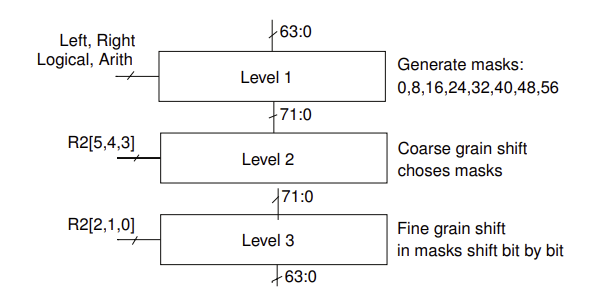
\includegraphics[scale = 0.8]
        {chapters/figures/T2Shifter}
        \caption{Black Box schematic of the T2 Shifter}
        \label{fig:T2Shifter}
        \end{figure}
    

    \subsection{ The Pentium 4 Adder}
    It is an efficient adder whose implementation is to minimize the critical path by making the bits of the operands that are being added or subtracted less vulnerable on 
    the carry bit propagation during the addition. Specifically, the adder is composed of two main blocks:

\begin{enumerate}
    \item The Carry Look Ahead Sparse Tree: It is a tree like structure formed of interconnected Propagate and Propagate-Generate blocks included for relying less on the dependency of the carry out done
    formed in a previous stages, for reduction of the critial path.
    \item The Carry Select Sum Block: similar to the carry look Ahead concept; it is formed of a sries of stages made of a specific predefined amount of concatenated full adders.
    Each stage has two parrallel chains of full adders  which perform respectively the addition on the hypothesis that the carry in bit is zero and one respectively.
    Then, the correct output of the addition between a particular subset of bits of the operands is chosen on the basis of the actual local carry produced by the sparse tree block described previously.
    
\end{enumerate}

    Summarizing, the adder/ subtractor module is implemented in a more efficient manner this way do to the fact that the addition of the particular subset of bits of the operands
    are all done in parallel unlike for instance the basic ripple carry adder model. Additionally, each set of ripple carry adders in the Carry Select Sum Block does not have to 
    wait for the carry out from the previous stage to perform the computation. Meaning that thanks to the Sparse tree, the addition/subtraction of the Pentium4 adder is more efficiently parallelized with respect to the addition
    performed by the Carry Look Ahead Adder model.

    Figure 5.3 depicts the block schematic of the described high level blocks which make up the pentium 4 adder module.

    \begin{figure}[h!]
        \centering
        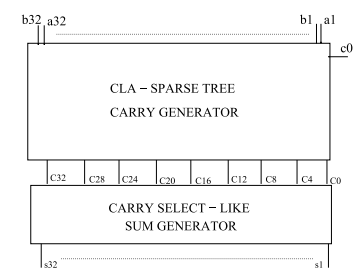
\includegraphics[scale = 1]
        {chapters/figures/Pentium4Adder}
        \caption{Black Box schematic of the Pentium 4 adder.}
        \label{fig:Pentium4Adder}
        \end{figure}

    \subsection{ The Comparator }
        The implemented comparator is constructed using the ouput of the present pentium four adder. Moreover, if two operands need to be compared,
        they will be firstly given to the pentium 4 block which will perform a subtraction. The comparator block will analize the carry out obtained from the results
        along with a flag bit called Z used set to one if the result of the subtraction is zero.
        Additionally the implemented comparator is able to perform a dual kind of operation in case the operands are treated as unisgned instead of signed.
        Figure 5.4 reports the schematic depicting the implementation of the comparator.

    \subsection{ The T2 Logicals }

    Logical instructions like the AND, OR and many others are performed through the T2 circuitry design. This choice was made as it leads
    to the implementation of a lot of logical operations still while using few gates (meaning less transistors equivalently). The structure is composed
    of four and gates in the fisrt level of the hirierchy. Then, the second level is one additional final and gate doing the and between the outputs of the first level.
    On the basis of the control bits of the dedicated to the execute phase there is the possibility to implement the logical operation of interest.
    Figure 5.4 depicts the circuit.

    \begin{figure}[h!]
        \centering
        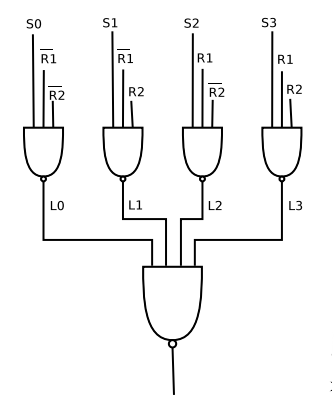
\includegraphics[scale = .6]
        {chapters/figures/T2Logic}
        \caption{The T2 Circuit for Logical Operations}
        \label{fig:T2Logic}
        \end{figure}

    For more details on the components specified above, chapter four from the Microelectronic Systems Lecture notes provides a more thorough analysis.
\newpage

\section{ Branch and Jump Related Circuitry }

The DLX sends out the selection signal for jumping in the fetch stage in the execution stage. Similarly, in case of a branch instruction,
the DLX determines whether the branch needs to be taken or not in the execution stage. the mechanism implemented for knowing if the branch and
jump need to be taken is composed of three multiplexers distributed hirierchically. In the first level of the hirierchy, there are two multiplexers.
one of them receives 1 and a signal called 'cond' (wich is the flag indicating if value stored the "REGA" pipe decode register is zero or not), and the other multiplexer has zero as first input 
and a signal called 'notCondIn' (which is the inversion of the of the CondIn signal ). The output of these two multiplexers are controled by one bit of the 
control unit which is one if the instruction is a Branch instruction, while when it is zero the instruction at analysis is not a branch. 
In the  second level of the hiriechy of the multiplexers there is one multiplexer which decides how to interpret the input it has (if it needs for instance
to branch do to an inequality of zero or do to an equality of zero.) Also for this second level of the multiplexer hiriechy there is a dedicated control bit from the  control unit.
Figure 5.5 depicts the multiplexer hiriechy that was discussed while Figure 5.6 is a table associating the control bits of interest to the various intructions

//INCLUDERE LE DUE FOTO APPENA FINITE


